\section{Pycnic}\label{pycnic}

\begin{figure}
\centering
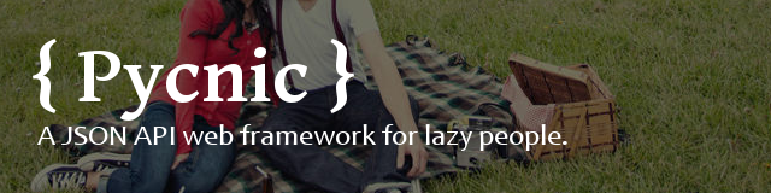
\includegraphics{images/pycnic}
\caption{Logo Pycnicu \autocite{pycnicpic}\label{pic:pycnic}}
\end{figure}

Pycnic je malý, rychlý a jednoduchý framework na tvorbu JSON API. Umí routovat, komunikovat v~JSONu a pracovat s~cookies \autocite{pycnic}. Pycnic neobsahuje žádné pokročilé funkce, ale ani je obsahovat nechce, jedná se opravdu o~minimalistickou knihovnu.

Pycnic je poměrně mladý projekt, který vnikl v~listopadu 2015. Jeho autorem je jednotlivec Aaron M., do kódu kromě něj nikdo nepřispěl\footnote{Pár jednotlivců přispělo do benchmarku, o~kterém bude řeč dále, nikoliv však do samotného kódu Pycnicu.}. Několik málo desítek hvězd na GitHubu také nasvědčuje tomu, že se zatím nejedná o~příliš známý projekt.

Pycnic závisí jen na standardní knihovně Pythonu. Instalace zabírá pouze 76 KiB a kód obsahuje pouhých 226 řádek, což je pro představu zhruba desetkrát více než kód \protect\hyperlink{code:pycnic}{v~ukázce}, ve které najdete příklad použití z~dokumentace.

Přestože Pycnic neobsahuje přímou podporu autentizace, v~dokumentaci poskytuje komplexní příklad, jak autentizaci implementovat \autocite{pycnicauth}. Kvůli jeho obsáhlosti jej zde neuvádím.

Vzhledem k~nízkoúrovnosti frameworku nedostává Pycnic v~žádném z~bodovaných kritérií body.

\begin{listing}[htbp]
\caption{{\label{code:pycnic}Příklad použití z~dokumentace Pycnicu \autocite{pycnicpost}}}
\begin{minted}[bgcolor=codebg]{python}
from pycnic.core import Handler, WSGI
from pycnic.errors import HTTP_400

class UsersHandler(Handler):

    def post(self):

        if not self.request.data.get("username"):
            raise HTTP_400("Yo dawg, you need to provide a username")

        return {
            "username":self.request.data["username"],
            "authID":self.request.cookies.get("auth_id"),
            "yourIp":self.request.ip,
            "rawBody":self.request.body,
            "method":self.request.method,
            "json":self.request.data,
            "XForward":self.request.environ["HTTP_X_FORWARDED_FOR"]
        }

class app(WSGI):
    routes = [ ("/user", UserHandler()) ]
\end{minted}
\end{listing}

\subsection{Benchmark}\label{benchmark}

Součástí repozitáře na GitHubu je i jednoduchý benchmark, který měří, kolik požadavků za sekundu jednotlivé webové frameworky zvládnou. Je měřena jednoduchá aplikace, která vrací na adrese \verb!/json! zprávu zakódovanou v~JSONu \autocite{pycnicbench}. Přestože se tato diplomová práce nezabývá webovými frameworky obecně, rozhodl jsem se měření provést. Ve výsledcích je kromě Pycnicu i Falcon a hug, které jsem zkoumal \protect\hyperlink{falcon}{v~části}, \protect\hyperlink{hug}{respektive}. Výsledky můžete vidět v~grafu \protect\hyperlink{pic:pycnicbench}{na obrázku}.

\begin{figure}
\centering
\includegraphics{pdfs/pycnic-chart}
\caption{Pycnic: Výsledky benchmarku\label{pic:pycnicbench}}
\end{figure}
